
In this subsection we use Zhuang's generalized \emph{run theorem} \cite{zhu16} to get two generating functions. Here ``run'' refers to a maximal weakly increasing consecutive subsequence in a word, so naturally this theorem suits the increasing pattern $\underline{123}$ the best. But according to Proposition~\ref{omega--omega^c}, finding the Eulerian distribution over $\underline{123}$-avoiding permutations is equivalent to finding the Eulerian distribution over $\underline{321}$-avoiding permutations. And the bivariate generating function for $\underline{321}$-avoiding permutations is already known to be \cite{MR06}

\begin{align}\label{Sn321des}
	\sum_{n\geq 0}\dfrac{x^n}{n!}\sum_{\pi \in S_n(\underline{321})} t^{\mathrm{des}(\pi)}=\dfrac{\mathrm{e}^{x/2}\sqrt{1-4t}}{\sqrt{1-4t}\cosh {\left(\frac{x}{2}\sqrt{1-4t}\right)}-\sinh{\left(\frac{x}{2}\sqrt{1-4t}\right)}}.
\end{align}
See also \cite[Thm.~5.3.4]{kit11}. Our proof of the following result could thus be viewed as an alternative approach to deriving \eqref{Sn321des}. We only sketch a proof here using the run theorem and illustrate the associated ``run network'' in Fig.~\ref{sn123runnetwork}. To make the paper self-contained however, we provide some preliminary definitions and facts in the Appendix, and the reader is referred to Zhuang's original paper~\cite{zhu16} for further information.

Note that a permuation $\pi$ avoids the consecutive pattern $\underline{123}$ if and only if each run of $\pi$ has length 1 or 2. Therefore, the corresponding run network is given by Fig.~\ref{sn123runnetwork}.

% , and we assign the weights $w_1^{(1 , 1)}=w_2^{(1,1)}=t$.

\begin{figure}[htbp]	
	 \centering
		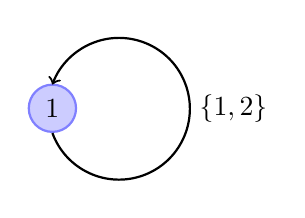
\begin{tikzpicture}
			[phase/.style ={circle,draw=blue!50,fill=blue!20,thick,inner sep=0pt, minimum size=6mm}]
			\node (A) at (0,-2) [phase] {1};
			\node (C) at (2.3,-2) {$\{1,2\}$};
			\draw[->,thick] (A.south) arc[start angle=-160, end angle=160, radius=9mm];
		\end{tikzpicture}
\caption{Run network for permutations avoiding consecutive pattern $\underline{123}$.}
\label{sn123runnetwork}
\end{figure}

\begin{theorem}
\begin{align}\label{Sn(123)des+1}
1+\sum_{n\geq 1}\dfrac{x^n}{n!}\sum_{\pi \in \S_n(\underline{123})} t^{\mathrm{des}(\pi)+1}=\dfrac{\mathrm{e}^{tx/2}\sqrt{t-4}}{\sqrt{t-4}\cosh {\left(\frac{x}{2}\sqrt{t^2-4t}\right)}-\sqrt{t}\sinh{\left(\frac{x}{2}\sqrt{t^2-4t}\right)}},
\end{align}
equivalently, we have
\begin{align}\label{Sn(123)des}
	\sum_{n\geq 0}\dfrac{x^n}{n!}\sum_{\pi \in \S_n(\underline{123})} t^{\mathrm{des}(\pi)}=\dfrac{t^{-1}\mathrm{e}^{tx/2}\sqrt{t-4}}{\sqrt{t-4}\cosh {\left(\frac{x}{2}\sqrt{t^2-4t}\right)}-\sqrt{t}\sinh{\left(\frac{x}{2}\sqrt{t^2-4t}\right)}}-\dfrac{1}{t}+1.
\end{align}
\end{theorem}

\begin{proof}
According to Fig.~\ref{sn123runnetwork} and applying Theorem~\ref{thm:gen run thm}, the inverse of $1+xt+x^2t$ is enumerator of those permutations whose increasing runs are no more than 2, and each increasing run is weighted by $t$. Next we proceed to seek the exponential generating function expression of $$\frac{1}{1+xt+x^2t}$$ with respect to the variable $x$. Since 
$$\dfrac{1}{1+xt+xt^2}=\dfrac{t-4+\sqrt{t^2-4t}}{2\left(t-4\right)}\dfrac{1}{1-\frac{2tx}{-t+\sqrt{t^2-4t}}}+\dfrac{t-4-\sqrt{t^2-4t}}{2(t-4)}\dfrac{1}{1-\frac{2tx}{-t-\sqrt{t^2-4t}}},$$ 
the exponential generating function turns out to be 
$$\frac{t-4+\sqrt{t^2-4t}}{2\left(t-4\right)} \mathrm{Exp}\left(\frac{-tx-x\sqrt{t^2-4t}}{2}\right)+\frac{t-4-\sqrt{t^2-4t}}{2\left(t-4\right)} \mathrm{Exp}\left(\frac{-tx+x\sqrt{t^2-4t}}{2}\right)$$
whose inverse simplifies to the desired expression \eqref{Sn(123)des+1}.
\end{proof}

% We note in passing that Eq.~\eqref{Sn(123)des} could be viewed as a bivariate extension of the expression of $P(0,z)$ in \cite[Thm.~4.1]{EN03}, which is the generating function of permutations avoiding $\underline{123}$.

%Note that $\pi^r \in \S_n(\underline{321})$ and $\mathrm{des}(\pi^r)=n-1-\mathrm{des}(\pi)$ if $\pi \in \S_n(123)$, consequently we have following result.
% By Proposition~\ref{omega--omega^c}, we immediately have the following result.
% \begin{corollary}	
% \begin{align}\label{Sn321des}
% 	\sum_{n\geq 0}\dfrac{x^n}{n!}\sum_{\pi \in S_n(\underline{321})} t^{\mathrm{des}(\pi)}=\dfrac{\mathrm{e}^{x/2}\sqrt{1-4t}}{\sqrt{1-4t}\cosh {\left(\frac{x}{2}\sqrt{1-4t}\right)}-\sinh{\left(\frac{x}{2}\sqrt{1-4t}\right)}}.
% \end{align}
% \end{corollary}
